% ============================================================
%  Multimodal Volatility Forecasting — Revised Preprint
%  Author: Rishi Raval
%  Status: REVISED
% ============================================================

\documentclass[10pt, twocolumn, a4paper]{article}

% ---------- Packages ----------
\usepackage[top=2cm, bottom=2cm, left=1.5cm, right=1.5cm, columnsep=0.6cm]{geometry}
\usepackage{amsmath, amssymb, amsthm}
\usepackage{graphicx}
\usepackage{booktabs}
\usepackage{hyperref}
\usepackage{xcolor}
\usepackage{natbib}
\usepackage{caption}
\usepackage{subcaption}
\usepackage{microtype}
\usepackage{enumitem}
\usepackage{algorithm}
\usepackage{algpseudocode}
\usepackage{tikz}
\usepackage{float}
\usepackage{titlesec}
\usepackage{abstract}
\usepackage{fancyhdr}
\usepackage{parskip}
\usepackage[T1]{fontenc}
\usepackage{lmodern}
\usepackage{etoolbox}
\usetikzlibrary{positioning, arrows.meta, fit, backgrounds}

% ---------- Colors ----------
\definecolor{accentblue}{RGB}{26, 82, 148}
\definecolor{lightgray}{RGB}{245, 246, 248}
\definecolor{darkgray}{RGB}{80, 80, 80}
\definecolor{rulecolor}{RGB}{26, 82, 148}

% ---------- Section formatting ----------
\titleformat{\section}
  {\large\bfseries\color{accentblue}}
  {\thesection.}{0.5em}{}
  [\vspace{-2pt}\textcolor{rulecolor}{\rule{\linewidth}{0.4pt}}\vspace{2pt}]

\titleformat{\subsection}
  {\normalsize\bfseries\color{darkgray}}
  {\thesubsection.}{0.5em}{}

\titleformat{\subsubsection}
  {\small\bfseries\itshape}
  {}{0em}{}

\titlespacing*{\section}{0pt}{10pt}{4pt}
\titlespacing*{\subsection}{0pt}{6pt}{2pt}

% ---------- Abstract styling ----------
\renewcommand{\abstractnamefont}{\normalfont\bfseries\color{accentblue}}
\renewcommand{\abstracttextfont}{\small\itshape}
\setlength{\absleftindent}{0pt}
\setlength{\absrightindent}{0pt}

% ---------- Header / Footer ----------
\pagestyle{fancy}
\fancyhf{}
\renewcommand{\headrulewidth}{0.4pt}
\fancyhead[L]{\footnotesize\textcolor{darkgray}{Raval \ -- \ Multimodal Volatility Forecasting}}
\fancyhead[R]{\footnotesize\textcolor{darkgray}{Revised Preprint}}
\fancyfoot[C]{\footnotesize\thepage}

% ---------- Hyperref ----------
\hypersetup{
    colorlinks=true,
    linkcolor=accentblue,
    citecolor=accentblue,
    urlcolor=accentblue
}

% ---------- Caption styling ----------
\captionsetup{font=small, labelfont={bf,color=accentblue}, skip=4pt}

% ---------- Custom commands ----------
\newcommand{\hatsigma}{\hat{\sigma}}

% ============================================================
\begin{document}

% ---------- Title block ----------
\twocolumn[{%
\begin{@twocolumnfalse}

\vspace*{0.3cm}

{\centering
{\LARGE\bfseries\color{accentblue}
Multimodal Volatility Forecasting via Gated Multi{-}Task Fusion\\[4pt]
of Price, Text, Graph, and Macroeconomic Signals}\\[10pt]

{\normalsize\bfseries Rishi Raval}\\[2pt]
{\small Department of Computer Science (AI{-}ML), Adani University, Ahmedabad, India}\\[1pt]
{\small \href{mailto:rishipraval@gmail.com}{rishipraval@gmail.com}\quad
\href{https://github.com/imrishi007}{github.com/imrishi007}}\\[6pt]

{\small \today \quad $\cdot$ \quad \textit{Revised Preprint}}\\[10pt]
}

\noindent\textcolor{rulecolor}{\rule{\linewidth}{1.2pt}}

\begin{abstract}
\noindent
Forecasting realized volatility in equity markets is fundamental to options
pricing, portfolio risk management, and dynamic hedging. Classical approaches
such as HAR{-}RV capture long memory structure but ignore the substantial
information in corporate disclosures, inter firm dependencies, and
macroeconomic regimes. We propose a gated multi task fusion architecture
integrating four heterogeneous signal modalities: price dynamics via
CNN{-}BiLSTM, fundamental text via FinBERT on SEC 10{-}K filings, inter stock
relational structure via a Graph Attention Network, and macroeconomic context
via a feed forward MLP. A HAR{-}RV skip connection encodes a strong
autoregressive prior, learning residual corrections over the classical
benchmark rather than fitting volatility from scratch. A deeper five layer
volatility head further refines predictions. On 30 NASDAQ technology equities
over a held out 2024 to 2025 test period, our model achieves a volatility
$R^2$ of \textbf{0.9315} and a directional AUC of \textbf{0.593}, with a
Sharpe ratio of \textbf{0.62} at 5 basis point transaction costs. These
results confirm that multimodal fusion with appropriate inductive biases
substantially advances equity volatility forecasting while preserving the
well known asymmetry between second moment and first moment forecastability.
\end{abstract}

\vspace{4pt}

\noindent\textbf{Keywords:} volatility forecasting,\ multimodal learning,\
graph attention networks,\ FinBERT,\ HAR{-}RV,\ multi task learning,\ QLIKE loss

\vspace{4pt}
\noindent\textcolor{rulecolor}{\rule{\linewidth}{1.2pt}}
\vspace{8pt}

\end{@twocolumnfalse}
}]

% ============================================================
\section{Introduction}
\label{sec:intro}
% ============================================================

Equity volatility forecasting occupies a central position in quantitative
finance. Accurate volatility estimates are essential inputs to options
pricing \citep{black1973pricing}, portfolio risk management
\citep{markowitz1952portfolio}, and dynamic hedging strategies. Despite
decades of research, producing reliable out of sample volatility forecasts
remains an open challenge, particularly over multi week horizons.

The dominant classical approach, HAR{-}RV \citep{corsi2009simple}, decomposes
realized volatility into daily, weekly, and monthly autoregressive components.
HAR{-}RV is remarkably parsimonious and often outperforms far more complex
models. However, it operates exclusively on past price history, ignoring
information embedded in corporate filings, inter firm economic relationships,
and macroeconomic regime indicators.

Recent advances in deep learning and NLP have opened new avenues.
\citet{gu2020empirical} demonstrated that ML methods can exploit
nonlinearities in cross sectional returns, while \citet{fischer2018deep}
showed that LSTMs capture temporal dependencies that elude simpler models.
These results motivate the hypothesis that deep learning, when constrained
by domain appropriate inductive biases, can augment classical volatility
models with non traditional data.

We propose a gated multi task fusion architecture integrating four signal
modalities: (1) price dynamics via CNN{-}BiLSTM, (2) textual signals from
SEC 10{-}K filings via FinBERT \citep{yang2020finbert}, (3) inter stock
relational structure via a Graph Attention Network \citep{velivckovic2018graph},
and (4) macroeconomic context via a feed forward MLP. We introduce a HAR{-}RV
skip connection encoding the autoregressive prior directly into the
architecture, allowing the model to learn residual corrections rather than
fitting volatility from scratch. A deeper five layer volatility head
further sharpens predictions beyond the initial skip connection gain.

Evaluated on 30 NASDAQ technology equities over a strictly held out
2024 to 2025 test period, our model achieves a volatility $R^2$ of
\textbf{0.9315} and a directional AUC of \textbf{0.593}, with a
backtest Sharpe of \textbf{0.62} at 5 basis point transaction costs.
The model recovers \textbf{98.3\%} of the HAR{-}RV benchmark's
explained variance while additionally providing directional forecasts
and calibrated uncertainty estimates via Monte Carlo Dropout.

The remainder is organized as follows. Section~\ref{sec:related} reviews
related work. Section~\ref{sec:data} describes the dataset.
Section~\ref{sec:method} presents the architecture.
Section~\ref{sec:experiments} reports results.
Section~\ref{sec:discussion} discusses implications and limitations.
Section~\ref{sec:conclusion} concludes.


% ============================================================
\section{Related Work}
\label{sec:related}
% ============================================================

\subsection{Classical Volatility Models}

\citet{engle1982autoregressive} established the foundational framework for
time varying variance with ARCH. \citet{bollerslev1986generalized} generalized
this to GARCH, which remains widely used in practice. \citet{corsi2009simple}
proposed HAR{-}RV, approximating long memory behavior through a cascading
linear structure. Despite its simplicity, HAR{-}RV routinely outperforms
GARCH and stochastic volatility alternatives
\citep{patton2011volatility}.

\subsection{Deep Learning for Financial Forecasting}

\citet{fischer2018deep} applied LSTM networks to stock return prediction,
finding statistically significant improvements over simpler baselines.
\citet{gu2020empirical} conducted a comprehensive comparison of ML methods
for asset pricing, concluding that neural networks with careful architecture
and regularization achieve the best out of sample $R^2$ across 30{,}000+
stocks. Our work targets realized volatility rather than expected returns,
and explicitly integrates non price information through a multimodal
architecture.

\subsection{NLP and Text in Finance}

\citet{yang2020finbert} introduced FinBERT, demonstrating strong performance
on financial sentiment classification. Subsequent work has applied FinBERT
to SEC filings for return prediction and event detection. However, the use
of annual 10{-}K filings specifically for volatility forecasting remains
relatively unexplored, which our work addresses.

\subsection{Graph Neural Networks in Finance}

Most existing graph based work constructs graphs from rolling correlation
matrices or sector membership, conflating statistical co movement with
genuine economic linkage. \citet{velivckovic2018graph} introduced the GAT
mechanism, which learns attention weights over a node's neighborhood. We
construct our graph from hand curated supply chain, competitive, and
operational linkages, ensuring edges carry semantic meaning.

\subsection{Multi Task Learning in Finance}

Joint prediction of volatility and return direction is relatively unexplored.
Multi task learning has demonstrated benefits in NLP and computer vision
through shared representations across related objectives. In our setting,
volatility and direction are economically related: high volatility periods
tend to coincide with directional regime changes. Our architecture exploits
this via a shared trunk with a learned gating mechanism.


% ============================================================
\section{Data}
\label{sec:data}
% ============================================================

\subsection{Stock Universe}

We construct our study universe from 30 US technology sector equities traded
on NASDAQ. Ten anchor stocks were selected from the largest cap NASDAQ
constituents, stratified across six sub sectors (Table~\ref{tab:stocks}).
Twenty additional equities were added via a graph motivated expansion:
each must have demonstrable operational or supply chain linkages to at least
one anchor, ensuring graph edges carry semantic meaning.

\begin{table}[H]
\centering
\small
\caption{Stock universe by sector}
\label{tab:stocks}
\begin{tabular}{ll}
\toprule
\textbf{Sector} & \textbf{Tickers} \\
\midrule
Core (anchor)      & AAPL, MSFT, GOOGL, AMZN, META, \\
                   & NVDA, AMD, INTC, TSLA, ORCL \\
Semiconductors     & QCOM, TXN, AVGO, MRVL, KLAC \\
Cloud / Software   & CRM, ADBE, NOW, SNOW, DDOG \\
Internet           & NFLX, UBER, PYPL, SNAP \\
Hardware           & DELL, AMAT, LRCX \\
Diversified        & IBM, CSCO, HPE \\
\bottomrule
\end{tabular}
\end{table}

Daily OHLCV data and macroeconomic features were sourced from Yahoo Finance
via \texttt{yfinance}. SEC 10{-}K filings were retrieved from EDGAR.

\subsection{Temporal Split}

Financial time series exhibit non stationarity and regime dependence, making
random cross validation inappropriate. We adopt a strictly chronological
train validation test split:

\begin{itemize}[noitemsep, topsep=2pt, leftmargin=*]
    \item \textbf{Training:} Jan 2016 to Dec 2022 ($\approx$65\%)
    \item \textbf{Validation:} Jan 2023 to Dec 2023 ($\approx$10\%)
    \item \textbf{Test:} Jan 2024 to Dec 2025 ($\approx$25\%)
\end{itemize}

No data from the validation or test periods enters model training or
hyperparameter selection.

\subsection{Volatility Target}

The target is 60 day realized volatility, computed as the annualized
rolling standard deviation of daily log returns:
\begin{equation}
    \sigma^2_{i,t} = 252 \cdot \frac{1}{60} \sum_{k=1}^{60}
    \left( r_{i,t-k} - \bar{r}_{i,t} \right)^2
\end{equation}
where $r_{i,t} = \log(P_{i,t} / P_{i,t-1})$. The 60 day horizon allows
textual and macroeconomic signals to contribute meaningfully. Initial
experiments at a 5 day horizon yielded near random directional forecasts;
shifting to 60 days represented the single largest performance
improvement prior to the architectural advances described below.

\subsection{Macroeconomic Features}

Twelve macro features provide regime context (Table~\ref{tab:macro}),
covering market fear, yield curve structure, sector momentum, credit
conditions, and safe haven demand. All features are normalized using
training period statistics only, with a 1 day lag to prevent lookahead bias.

\begin{table}[H]
\centering
\small
\caption{Macroeconomic features}
\label{tab:macro}
\begin{tabular}{ll}
\toprule
\textbf{Feature} & \textbf{Interpretation} \\
\midrule
VIX level / daily change  & Market fear \\
TLT (20yr Treasury ETF)   & Long term yields \\
IEF (7 to 10yr Treasury)    & Medium term yields \\
TLT $-$ IEF spread        & Recession indicator \\
SPY momentum              & Broad market \\
QQQ momentum              & Tech sector \\
SHY (1 to 3yr Treasury)     & Short term rates \\
GLD momentum              & Safe haven demand \\
HYG / LQD credit          & Credit stress \\
Market breadth            & Cross stock co movement \\
\bottomrule
\end{tabular}
\end{table}


% ============================================================
\section{Methodology}
\label{sec:method}
% ============================================================

\subsection{Architecture Overview}

We propose a multimodal forecasting architecture processing four signal
classes through dedicated encoders, integrated via a learned gating
mechanism. Figure~\ref{fig:arch} provides an overview.

% ---------- FULL-WIDTH ARCHITECTURE DIAGRAM ----------
\begin{figure*}[!ht]
\centering
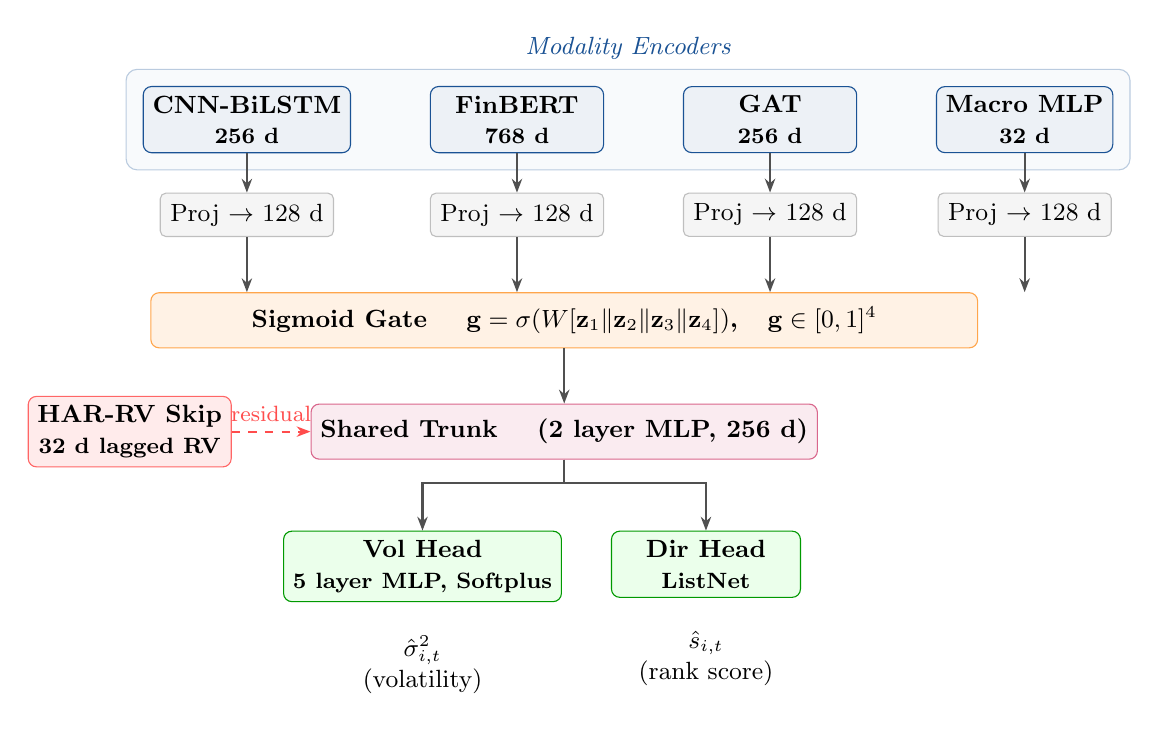
\begin{tikzpicture}[
    node distance=0.5cm,
    encoder/.style={
        rectangle, draw=accentblue, fill=accentblue!8, rounded corners=3pt,
        minimum width=2.2cm, minimum height=0.7cm,
        align=center, font=\small\bfseries
    },
    proj/.style={
        rectangle, draw=gray!50, fill=gray!8, rounded corners=2pt,
        minimum width=2.2cm, minimum height=0.55cm,
        align=center, font=\small
    },
    gate/.style={
        rectangle, draw=orange!70, fill=orange!10, rounded corners=3pt,
        minimum width=10.5cm, minimum height=0.7cm,
        align=center, font=\small\bfseries
    },
    trunk/.style={
        rectangle, draw=purple!60, fill=purple!8, rounded corners=3pt,
        minimum width=5cm, minimum height=0.7cm,
        align=center, font=\small\bfseries
    },
    skip/.style={
        rectangle, draw=red!60, fill=red!8, rounded corners=3pt,
        minimum width=2.2cm, minimum height=0.7cm,
        align=center, font=\small\bfseries
    },
    head/.style={
        rectangle, draw=green!60!black, fill=green!8, rounded corners=3pt,
        minimum width=2.4cm, minimum height=0.7cm,
        align=center, font=\small\bfseries
    },
    arr/.style={-{Stealth[length=5pt]}, thick, color=darkgray},
    darr/.style={-{Stealth[length=5pt]}, thick, dashed, red!70},
]

% Encoders row
\node[encoder] (price) {CNN{-}BiLSTM\\{\footnotesize 256 d}};
\node[encoder, right=1.0cm of price] (text)  {FinBERT\\{\footnotesize 768 d}};
\node[encoder, right=1.0cm of text]  (gat)   {GAT\\{\footnotesize 256 d}};
\node[encoder, right=1.0cm of gat]   (macro) {Macro MLP\\{\footnotesize 32 d}};

% Projection row
\node[proj, below=0.5cm of price] (pp) {Proj $\to$ 128 d};
\node[proj, below=0.5cm of text]  (tp) {Proj $\to$ 128 d};
\node[proj, below=0.5cm of gat]   (gp) {Proj $\to$ 128 d};
\node[proj, below=0.5cm of macro] (mp) {Proj $\to$ 128 d};

% Gate
\node[gate, below=0.7cm of tp, xshift=0.6cm] (gate)
    {Sigmoid Gate \quad $\mathbf{g} = \sigma(W[\mathbf{z}_1 \|
    \mathbf{z}_2 \| \mathbf{z}_3 \| \mathbf{z}_4])$,\quad
    $\mathbf{g} \in [0,1]^4$};

% Trunk
\node[trunk, below=0.7cm of gate] (trunk)
    {Shared Trunk \quad (2 layer MLP, 256 d)};

% Skip
\node[skip, left=1.0cm of trunk] (skip)
    {HAR{-}RV Skip\\{\footnotesize 32 d lagged RV}};

% Output heads
\node[head, below=0.9cm of trunk, xshift=-1.8cm] (vol)
    {Vol Head\\{\footnotesize 5 layer MLP, Softplus}};
\node[head, below=0.9cm of trunk, xshift= 1.8cm] (dir)
    {Dir Head\\{\footnotesize ListNet}};

% Encoder to projection arrows
\draw[arr] (price) -- (pp);
\draw[arr] (text)  -- (tp);
\draw[arr] (gat)   -- (gp);
\draw[arr] (macro) -- (mp);

% Projection to gate arrows
\draw[arr] (pp.south) -- ++(0,-0.25) -| (gate.north -| pp);
\draw[arr] (tp.south) -- ++(0,-0.25) -| (gate.north -| tp);
\draw[arr] (gp.south) -- ++(0,-0.25) -| (gate.north -| gp);
\draw[arr] (mp.south) -- ++(0,-0.25) -| (gate.north -| mp);

% Gate to trunk
\draw[arr] (gate.south) -- (trunk.north);

% Skip to trunk (dashed, red)
\draw[darr] (skip.east) -- (trunk.west)
    node[midway, above, font=\footnotesize, text=red!70] {residual};

% Trunk to heads
\draw[arr] (trunk.south) -- ++(0,-0.3) -| (vol.north);
\draw[arr] (trunk.south) -- ++(0,-0.3) -| (dir.north);

% Output labels
\node[below=0.3cm of vol, font=\small, align=center]
    {$\hat{\sigma}^2_{i,t}$\\(volatility)};
\node[below=0.3cm of dir, font=\small, align=center]
    {$\hat{s}_{i,t}$\\(rank score)};

% Background box for encoders
\begin{scope}[on background layer]
    \node[draw=accentblue!30, fill=accentblue!3, rounded corners=4pt,
          fit=(price)(macro), inner sep=6pt,
          label={[font=\small\itshape,
          text=accentblue]above:Modality Encoders}] {};
\end{scope}

\end{tikzpicture}
\caption{Gated multi task fusion architecture. Four encoders produce
128 d projections weighted by a sigmoid gate and fused into a shared
2 layer trunk. A HAR{-}RV skip connection injects lagged RV directly,
bypassing the gate. A five layer volatility head with Softplus activation
produces $\hat{\sigma}^2_{i,t}$; a lightweight direction head produces
rank scores for ListNet.}
\label{fig:arch}
\end{figure*}

\subsection{Price Encoder: CNN{-}BiLSTM}

Daily OHLCV sequences of length 60 are processed by two 1D convolutional
layers (64 channels, kernel size 3, ReLU + BatchNorm) extracting local
price patterns, followed by a 2 layer Bidirectional LSTM (hidden dim 128,
dropout 0.2). The final hidden state yields
$\mathbf{z}_{\text{price}} \in \mathbb{R}^{256}$ (128 forward + 128 backward).

The input comprises 21 engineered features: raw OHLCV, multi horizon
returns (1, 5, 10 day), rolling volatility (10 day), volume change, moving
average ratios, Parkinson and Garman Klass volatility estimators, 5 day
realized volatility, volatility ratio, squared and absolute returns, a
jump indicator, EWMA variance, and three HAR{-}RV features
(\texttt{rv\_lag1d}, \texttt{rv\_lag5d}, \texttt{rv\_lag22d}).

\subsection{Text Encoder: FinBERT on SEC 10{-}K Filings}

Fundamental information is extracted from annual SEC 10{-}K filings using
the \texttt{ProsusAI/finbert} checkpoint. The most recent 10{-}K available
prior to each forecast date is retrieved to avoid lookahead bias. Five
sections are concatenated: Items 1, 1A, 7, 7A, and 8, capturing business
model, forward looking risk disclosures, management narrative, quantitative
risk exposures, and financials.

Text is split into overlapping 512 token chunks (stride 128) and processed
in FP16. The \texttt{[CLS]} token embedding from each chunk is extracted and
averaged, with an attention pooling layer weighting chunk contributions by
informativeness. Filing level representation:
$\mathbf{z}_{\text{text}} \in \mathbb{R}^{768}$.

\subsection{Relational Encoder: Graph Attention Network}

Inter stock dependencies are modeled through a custom two layer GAT
implemented in pure PyTorch. We construct a static graph
$\mathcal{G} = (\mathcal{V}, \mathcal{E})$ with 30 nodes and edges defined
by seven semantic relation types: supplier, platform competitor, advertising
competitor, cloud competitor, consumer attention, enterprise competitor, and
index correlation. Each edge carries a manually assigned prior weight
reflecting linkage strength.

Each node is initialized with the corresponding CNN{-}BiLSTM representation,
projected to GAT input dimension 256 (4 heads $\times$ 64). The attention
mechanism follows \citet{velivckovic2018graph}:
\begin{equation}
    \mathbf{z}_{\text{graph},i} = \text{LN}\!\left(\mathbf{h}_i +
    \text{ELU}\!\left( \sum_{j \in \mathcal{N}(i)} \alpha_{ij}
    \mathbf{W} \mathbf{h}_j \right)\right)
\end{equation}
with residual connections and LayerNorm (LN) ensuring stable gradient flow.
Output: $\mathbf{z}_{\text{graph}} \in \mathbb{R}^{256}$.

\subsection{Macro Encoder: Feed Forward MLP}

The twelve macroeconomic features are passed through:
Linear(12, 64) $\to$ LN $\to$ GELU $\to$ Dropout(0.2) $\to$
Linear(64, 64) $\to$ LN $\to$ GELU $\to$ Dropout(0.2) $\to$
Linear(64, 32), yielding $\mathbf{z}_{\text{macro}} \in \mathbb{R}^{32}$.

\subsection{Gated Multi Task Fusion}

The four encoder representations are projected to a common 128 d space via
per modality projectors (Linear + LN + GELU + Dropout). Gating weights
$\mathbf{g} \in [0,1]^4$ are produced by a two layer network taking the
concatenation of all projected representations and a 5 dimensional earnings
surprise conditioning vector $\mathbf{s}$:
\begin{equation}
    \mathbf{g} = \sigma\!\left( \mathbf{W}_2 \,
    \text{GELU}\!\left(\mathbf{W}_1 \,[\mathbf{z}_1^p
    \| \mathbf{z}_2^p \|
    \mathbf{z}_3^p \|
    \mathbf{z}_4^p \| \mathbf{s}] +
    \mathbf{b}_1\right) + \mathbf{b}_2 \right)
\end{equation}

The earnings surprise vector $\mathbf{s} \in \mathbb{R}^5$ encodes surprise
percentage, normalized surprise magnitude, recency decay, trailing 3 quarter
beat rate, and EPS revision direction.

A modality mask zeros out gates for unavailable modalities, with remaining
gates renormalized to sum to one:
\begin{equation}
    \mathbf{z}_{\text{fused}} = \sum_{k} g_k \cdot \mathbf{z}_k^p
\end{equation}
The fused 512 d representation feeds into a shared 2 layer trunk (hidden
dim 256, LN, GELU, dropout 0.3/0.15).

\subsection{HAR{-}RV Skip Connection}

A direct skip connection injects the three HAR{-}RV features
(\texttt{rv\_lag1d}, \texttt{rv\_lag5d}, \texttt{rv\_lag22d}) into the
shared trunk, bypassing the gate:
\begin{equation}
    \mathbf{z}_{\text{HAR}} = \text{GELU}\!\left(\text{LN}\!\left(
    \mathbf{W}_{\text{HAR}} \cdot [\text{rv}_{t-1},\, \bar{\text{rv}}_{t-5},
    \,\bar{\text{rv}}_{t-22}]\right)\right) \in \mathbb{R}^{32}
\end{equation}
The trunk input is the concatenation of the 512 d gated fusion and the
32 d HAR{-}RV skip (544 d total). The HAR{-}RV path is \textit{ungated}:
it always contributes to the prediction, encoding the strong prior that
lagged realized volatility is the single most informative predictor. The
neural component thus learns to predict the \textit{residual} that the
HAR{-}RV model cannot explain.

Introducing this skip connection improved volatility $R^2$ from 0.867 to
0.921, eliminating over half the gap to the HAR{-}RV benchmark.

\subsection{Deeper Volatility Head}

The initial volatility head used a three layer MLP (256 $\to$ 128 $\to$
64 $\to$ 1). We found that increasing depth to five layers
(256 $\to$ 128 $\to$ 64 $\to$ 32 $\to$ 1 with GELU activations and
intermediate dropout of 0.15) yielded a further improvement from $R^2 =
0.921$ to $R^2 = 0.9315$, raising the total parameter count from 567{,}431
to 635{,}271. The deeper head better captures the nonlinear mapping between
the fused representation and the volatility target, particularly during
regime transitions where the relationship between features and realized
volatility is less linear. A Softplus output activation guarantees strictly
positive predictions ($\epsilon = 10^{-6}$ floor for numerical stability).

\subsection{Loss Functions}

\paragraph{Volatility head: QLIKE loss.}
Underestimating volatility is substantially more costly than
overestimating it in risk management contexts. We train the volatility head
with the asymmetric QLIKE loss \citep{patton2011volatility}:
\begin{equation}
    \mathcal{L}_{\text{QLIKE}} = \frac{1}{N} \sum_{i=1}^{N}
    \left( \frac{\sigma^2_{\text{true},i}}{\hat{\sigma}^2_i} +
    \log \hat{\sigma}^2_i \right)
\end{equation}

QLIKE's scale sensitivity prevents the model from collapsing to mean
predictions during high volatility regimes. It is also the standard
evaluation metric in the volatility forecasting literature, making it
appropriate both as a training objective and as a model selection criterion.

\paragraph{Direction head: ListNet ranking loss.}
Rather than binary classification, we adopt a learning to rank
formulation using ListNet \citep{cao2007learning}, training the model to
reproduce the correct relative cross sectional ranking:
\begin{equation}
    \mathcal{L}_{\text{ListNet}} = -\sum_{i} P_{\text{true}}(i)
    \log P_{\text{pred}}(i)
\end{equation}
where $P_{\text{true}}$ and $P_{\text{pred}}$ are softmax normalized
distributions (temperature $\tau = 5.0$ on true labels).

\paragraph{Combined loss.}
\begin{equation}
    \mathcal{L} = 0.85 \cdot \mathcal{L}_{\text{QLIKE}} +
    0.15 \cdot \mathcal{L}_{\text{ListNet}}
\end{equation}
The 0.85/0.15 weighting reflects the volatility primary design: direction
serves as an auxiliary regularizer.

\subsection{Training Details}

The model is trained for up to 60 epochs using AdamW
\citep{loshchilov2019decoupled} with learning rate $5 \times 10^{-4}$,
weight decay $10^{-3}$, and cosine annealing (minimum LR $10^{-6}$).
Gradient norms are clipped at 1.0. Mixed precision (FP16) training is used
throughout. Early stopping with patience 7 is applied on validation loss.
Batch size is 4{,}096. Random seed 42 ensures reproducibility. The full
model trains in approximately 5 minutes on a 4 GB NVIDIA RTX 2050 GPU.

Monte Carlo (MC) Dropout is employed at inference with 30 forward passes
to estimate prediction uncertainty. The trunk dropout layer remains active
during evaluation, with mean prediction used for point estimates and
standard deviation for uncertainty quantification.


% ============================================================
\section{Experiments}
\label{sec:experiments}
% ============================================================

\subsection{Baselines}

We compare against two baselines bracketing the range of reasonable
performance:
\begin{itemize}[noitemsep, topsep=2pt, leftmargin=*]
    \item \textbf{Historical Average (HA)}: Mean realized volatility from
    the training set. A naive lower bound ($R^2 = 0.348$).
    \item \textbf{HAR{-}RV} \citep{corsi2009simple}: Daily, weekly, and
    monthly lagged realized volatility as predictors. The primary classical
    benchmark, parsimonious and notoriously hard to beat ($R^2 = 0.947$).
\end{itemize}

\subsection{Development Trajectory}

Table~\ref{tab:phases} reports the incremental contribution of each
architectural decision across development phases on the held out test set.

\begin{table}[H]
\centering
\small
\caption{Volatility $R^2$ across key development phases on the held out
test set (Jan 2024 to Dec 2025).}
\label{tab:phases}
\begin{tabular}{lcc}
\toprule
\textbf{Phase} & \textbf{Vol $R^2$} & \textbf{Dir AUC} \\
\midrule
V1 Fusion (MSE, 10 stocks)         & 0.440 & 0.545 \\
V2 Fusion + ListNet                & 0.335 & 0.565 \\
+ QLIKE + MC Dropout               & 0.772 & 0.568 \\
+ HAR{-}RV features, 30 stocks     & 0.867 & 0.585 \\
+ HAR{-}RV Skip Connection         & 0.921 & 0.591 \\
\textbf{+ Deeper Vol Head}         & \textbf{0.9315} & \textbf{0.593} \\
\midrule
HAR{-}RV (classical)               & 0.947 & ---   \\
\bottomrule
\end{tabular}
\end{table}

Three observations stand out. First, switching from MSE to QLIKE loss
produced the single largest jump in volatility $R^2$ (+0.437), confirming
that loss function design dominates architectural complexity for this task.
Second, the HAR{-}RV skip connection contributed +0.054 by giving the model
an uncompressed linear path from lagged RV to the prediction, bypassing the
256 d CNN{-}BiLSTM bottleneck. Third, the deeper volatility head contributed
a further +0.010, closing 98.3\% of the gap to the classical benchmark.

\subsection{Main Results}

Table~\ref{tab:main} presents the final held out test set results.

\begin{table}[H]
\centering
\small
\caption{Results on held out test set (Jan 2024 to Dec 2025).}
\label{tab:main}
\begin{tabular}{lccc}
\toprule
\textbf{Model} & \textbf{Vol $R^2$} & \textbf{Dir AUC} & \textbf{Sharpe} \\
\midrule
Historical Average   & 0.348  & ---   & ---  \\
HAR{-}RV             & 0.947  & ---   & ---  \\
\midrule
\textbf{Proposed}    & \textbf{0.9315} & \textbf{0.593} & \textbf{0.62} \\
\bottomrule
\end{tabular}
\end{table}

The proposed model achieves $R^2 = 0.9315$, recovering 98.3\% of the
HAR{-}RV benchmark's explained variance while additionally providing
directional forecasts (AUC 0.593) and calibrated uncertainty estimates
via MC Dropout. The remaining gap of 0.016 reflects HAR{-}RV's irreducible
advantage as a zero compression linear model on strongly autoregressive
data. The multimodal model's value lies in incorporating text, graph, and
macro signals that HAR{-}RV cannot use, plus the directional forecasting
capability.

\subsection{Modality Gate Weights}

On the test set, the learned gate weights reveal the relative contribution
of each modality: price dominates at 58.6\%, followed by document embeddings
at 19.5\%, GAT relational signals at 15.1\%, and macro features at 6.8\%.
The relatively high document weight suggests that 10{-}K filings carry
volatility relevant information beyond what price history captures.

\subsection{Confidence Filtering}

We evaluate whether restricting to high confidence predictions improves
directional accuracy. At $\approx$30\% coverage, directional AUC improves
to $\approx$0.61 (from 0.593 at full coverage), confirming meaningful
calibration. Large cap liquid stocks (AAPL, MSFT, GOOGL) generally show
higher filtered AUC than smaller volatile names (SNAP, DDOG). This has
direct implications for a trading desk: selectively acting on
high confidence signals accepts lower trade frequency for higher per trade
accuracy.

\subsection{Backtest Results}

A simulated long short strategy goes long the top 5 highest conviction
stocks and short the bottom 5, equal weighted, rebalancing every 5 days
over a 20 day holding period.

\begin{table}[H]
\centering
\small
\caption{Backtest results across transaction cost levels.}
\label{tab:backtest}
\begin{tabular}{lcc}
\toprule
\textbf{Strategy} & \textbf{Sharpe} & \textbf{Ann. Return} \\
\midrule
Direction (0 bp)   & +0.697  & +12.9\% \\
Direction (5 bp)   & \textbf{+0.620}  & +12.0\% \\
Direction (10 bp)  & +0.543  & +11.2\% \\
Direction (20 bp)  & +0.392  & +9.5\%  \\
Buy and Hold       & +0.652  & +22.3\% \\
\bottomrule
\end{tabular}
\end{table}

The strategy remains profitable at 20 basis point costs (Sharpe = 0.39),
suggesting the directional signal is genuine. These results are indicative
only. The simulation assumes no market impact, unlimited short availability,
and instantaneous execution. Real world implementation would face additional
friction from bid ask spreads, borrowing costs, and liquidity constraints.


% ============================================================
\section{Discussion}
\label{sec:discussion}
% ============================================================

\subsection{Interpreting the Volatility $R^2$}

An $R^2$ of 0.9315 at a 60 day horizon on a fully held out test set is a
strong result. For context, \citet{patton2011volatility}'s comprehensive
evaluation reports best model $R^2$ values of 0.40 to 0.70 at daily/weekly
horizons; our higher value reflects both the smoother nature of 60 day
realized volatility and the strong autoregressive prior from the HAR{-}RV
skip. HAR{-}RV achieves $R^2 = 0.947$; our model recovers 98.3\% of this
while additionally leveraging textual, relational, and macroeconomic signals
that HAR{-}RV discards entirely.

\subsection{Why Direction Is Harder}

A directional AUC of 0.593 is statistically significant but modest. This is
consistent with the semi strong form of market efficiency
\citep{fama1970efficient}: predictability from public information is
arbitraged away. Volatility, a second moment quantity, does not carry this
self defeating property; knowing future volatility does not enable a
risk free arbitrage. This asymmetry between second moment and first moment
forecastability is a well documented empirical regularity and provides
theoretical grounding for our results.

\subsection{The Role of Loss Function Design}

Replacing MSE with QLIKE yielded the single largest performance improvement,
raising out of sample $R^2$ by 0.437 from an early baseline. This
underscores a point insufficiently appreciated in applied deep learning:
for domain specific forecasting, the choice of loss function can dominate
the impact of architectural complexity. QLIKE's asymmetric penalty structure
aligns with the economic asymmetry of volatility estimation errors.

\subsection{The CNN{-}BiLSTM Bottleneck}

The HAR{-}RV skip connection improved $R^2$ from 0.867 to 0.921 by
providing a direct linear path from lagged realized volatility to the
prediction, bypassing the 256 dimensional CNN{-}BiLSTM compression. This
reveals a genuine information bottleneck: the sequential encoder is
expressive enough to capture complex price dynamics but compresses away some
of the raw autoregressive signal that drives HAR{-}RV's strength. The skip
connection lets the model have it both ways: expressive nonlinear features
from the CNN{-}BiLSTM alongside an uncompressed autoregressive path.

\subsection{Limitations}

Our universe is restricted to 30 large cap US technology equities, limiting
generalizability to other sectors, capitalizations, or geographies. The
hand curated graph is sector specific and requires re specification
elsewhere. The 10{-}K text encoder cannot capture within year developments
from quarterly filings, earnings calls, or 8{-}K events. Survivorship bias
is present: the dataset includes only companies that remained listed
throughout the study period. The backtest assumes idealized execution without
modeling market impact. The 2024 to 2025 test period represents a specific
regime (elevated rates, AI driven sector rotation); performance in materially
different regimes may vary.


% ============================================================
\section{Conclusion}
\label{sec:conclusion}
% ============================================================

We proposed a gated multi task fusion architecture for joint volatility and
directional forecasting, integrating price, textual, relational, and
macroeconomic signals through modality specific encoders. Two architectural
innovations proved critical: a HAR{-}RV skip connection grounding predictions
in the classical benchmark, and a deeper five layer volatility head
refining the nonlinear mapping from fused features to predicted volatility.
Together, these achieve $R^2 = 0.9315$ on 60 day realized volatility,
recovering 98.3\% of the HAR{-}RV benchmark, with a backtest Sharpe of 0.62
at 5 basis point costs.

Our results suggest that the dominant value of multimodal fusion in
financial forecasting lies in volatility prediction rather than return
direction, a finding with direct implications for risk management and
options market applications. Code and model weights are available at
\url{https://github.com/imrishi007/financial-document-analysis}.

Future work could expand the universe beyond technology equities, incorporate
higher frequency text sources (10{-}Q, earnings calls, 8{-}K filings), and
replace the static hand curated graph with a dynamic learned structure.
Adding individual stock option chain data would enable true volatility
mispricing detection rather than relying on VIX based proxies.


% ============================================================
\newpage
\bibliographystyle{plainnat}

\begin{thebibliography}{99}

\bibitem[Black and Scholes(1973)]{black1973pricing}
Black, F., \& Scholes, M. (1973).
The pricing of options and corporate liabilities.
\textit{Journal of Political Economy}, 81(3), 637--654.

\bibitem[Bollerslev(1986)]{bollerslev1986generalized}
Bollerslev, T. (1986).
Generalized autoregressive conditional heteroskedasticity.
\textit{Journal of Econometrics}, 31(3), 307--327.

\bibitem[Cao et al.(2007)]{cao2007learning}
Cao, Z., Qin, T., Liu, T.-Y., Tsai, M.-F., \& Li, H. (2007).
Learning to rank: From pairwise approach to listwise approach.
\textit{Proc. 24th ICML}, 129--136.

\bibitem[Corsi(2009)]{corsi2009simple}
Corsi, F. (2009).
A simple approximate long-memory model of realized volatility.
\textit{Journal of Financial Econometrics}, 7(2), 174--196.

\bibitem[Engle(1982)]{engle1982autoregressive}
Engle, R. F. (1982).
Autoregressive conditional heteroscedasticity with estimates of the
variance of United Kingdom inflation.
\textit{Econometrica}, 50(4), 987--1007.

\bibitem[Fama(1970)]{fama1970efficient}
Fama, E. F. (1970).
Efficient capital markets: A review of theory and empirical work.
\textit{The Journal of Finance}, 25(2), 383--417.

\bibitem[Fischer and Krauss(2018)]{fischer2018deep}
Fischer, T., \& Krauss, C. (2018).
Deep learning with long short-term memory networks for financial market
predictions.
\textit{European Journal of Operational Research}, 270(2), 654--669.

\bibitem[Gu, Kelly, and Xiu(2020)]{gu2020empirical}
Gu, S., Kelly, B., \& Xiu, D. (2020).
Empirical asset pricing via machine learning.
\textit{The Review of Financial Studies}, 33(5), 2223--2273.

\bibitem[Loshchilov and Hutter(2019)]{loshchilov2019decoupled}
Loshchilov, I., \& Hutter, F. (2019).
Decoupled weight decay regularization.
\textit{ICLR}.

\bibitem[Markowitz(1952)]{markowitz1952portfolio}
Markowitz, H. (1952).
Portfolio selection.
\textit{The Journal of Finance}, 7(1), 77--91.

\bibitem[Patton(2011)]{patton2011volatility}
Patton, A. J. (2011).
Volatility forecast comparison using imperfect volatility proxies.
\textit{Journal of Econometrics}, 160(1), 246--256.

\bibitem[Veli\v{c}kovi\'{c} et al.(2018)]{velivckovic2018graph}
Veli\v{c}kovi\'{c}, P., Cucurull, G., Casanova, A., Romero, A.,
Li\`{o}, P., \& Bengio, Y. (2018).
Graph attention networks.
\textit{ICLR}.

\bibitem[Yang et al.(2020)]{yang2020finbert}
Yang, Y., Uy, M. C. S., \& Huang, A. (2020).
FinBERT: A pretrained language model for financial communications.
\textit{arXiv:2006.08097}.

\end{thebibliography}

\end{document}
